\chapter{Hello World}

It is now time for us to start practicing coding skills.
In this course, we will be focusing on learning how to program
in Java, which is just one of many programming languages.
While each programming language has its own quirks and features
specific to it, many of the concepts you will learn in this
class will exist not only in Java but also in other languages.

We will now write our first program in Java called ``Hello World.''
We will use DrJava to help us write, compile, and run this program.

\section{Starting DrJava}
TODO: how to start DrJava on laptop that students are given

TODO: add screenshot of DrJava when just opened and label parts


On the left-hand side of the window, there is a list of currently-open files. When you first start up DrJava, the only thing there should say ``(Untitled)''.
The main part of the window is where you will write code.

TODO: add instructions on adding line numbers on student laptop.

There should be numbers along the left-hand side to make it easy for you to see which line you are writing code on. The bottom part of the window is where we can interact with the program, for example by seeing the output of compiling the program or by seeing the output of running the program.

\section{Writing Hello World}

In the main part of the window, type the following code:
\begin{code}
class HelloWorld {
    
    public static void main(String[] args) {
        System.out.println("Hello World!");
    }
    
}
\end{code}

We will learn more about what the different parts of this program do later. Here is a brief explanation for now:
\begin{enumerate}
\item In line 1, \ic{class HelloWorld} makes a new \emph{class} called \ic{HelloWorld}. In Java, all code must be enclosed in a class. The class contains all the code between the open curly brace \ic{\{} on line 1 and the close curly brace \ic{\}} on line 7.
\item Line 3 makes a new ``method" called \ic{main}. We will learn later what
\ic{public static void} and \ic{String[] args} mean. For now, all you
need to know is that every Java program needs a \ic{main} method.
% and starts
% by executing the code within the \ic{main} method. Our \ic{main} method
% contains all the code between the open curly brace \ic{\{} on line 3 and the
% close curly brace \ic{\}} on line 5.
\item Line 4 is a print statement. \ic{System.out.println} will print out
whatever is specified between the open parenthesis \ic{(} and closed
parenthesis\ic{)} that follows immediately after.
% \ic{System.out.println} will begin a new line after printing out whatever is specified in the parentheses.
% In this case, we
% put the \emph{string literal} \ic{"Hello World!"} in between these parentheses.
% String literals refer to text between quotation marks.
\end{enumerate}

Our explanation is summarized in the following graphic.

\begin{figure}[ht]
	\centering
	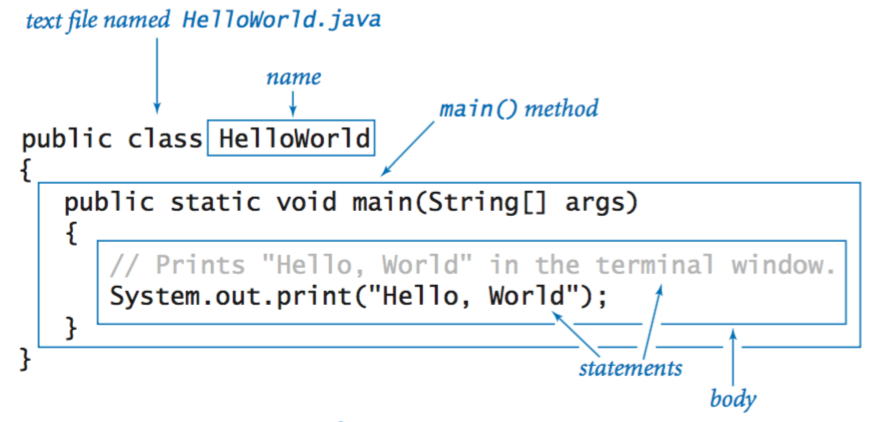
\includegraphics[width=0.85\textwidth]{images/hello.png}
% 	\caption{Creating a CS103 folder inside your Desktop.}
	\label{fig:helloworld:example}
\end{figure}


\section{Saving and Compiling in DrJava}

In the upper part of the window, you should see a toolbar with many buttons.
You can now click the ``Save'' button. 

First, navigate to your Desktop folder. Once there, create a new folder called CS103 (see Figure \ref{fig:helloworld:sec:saving}). We will store all of our files for the semester in this folder. 

\begin{figure}[ht]
	\centering
	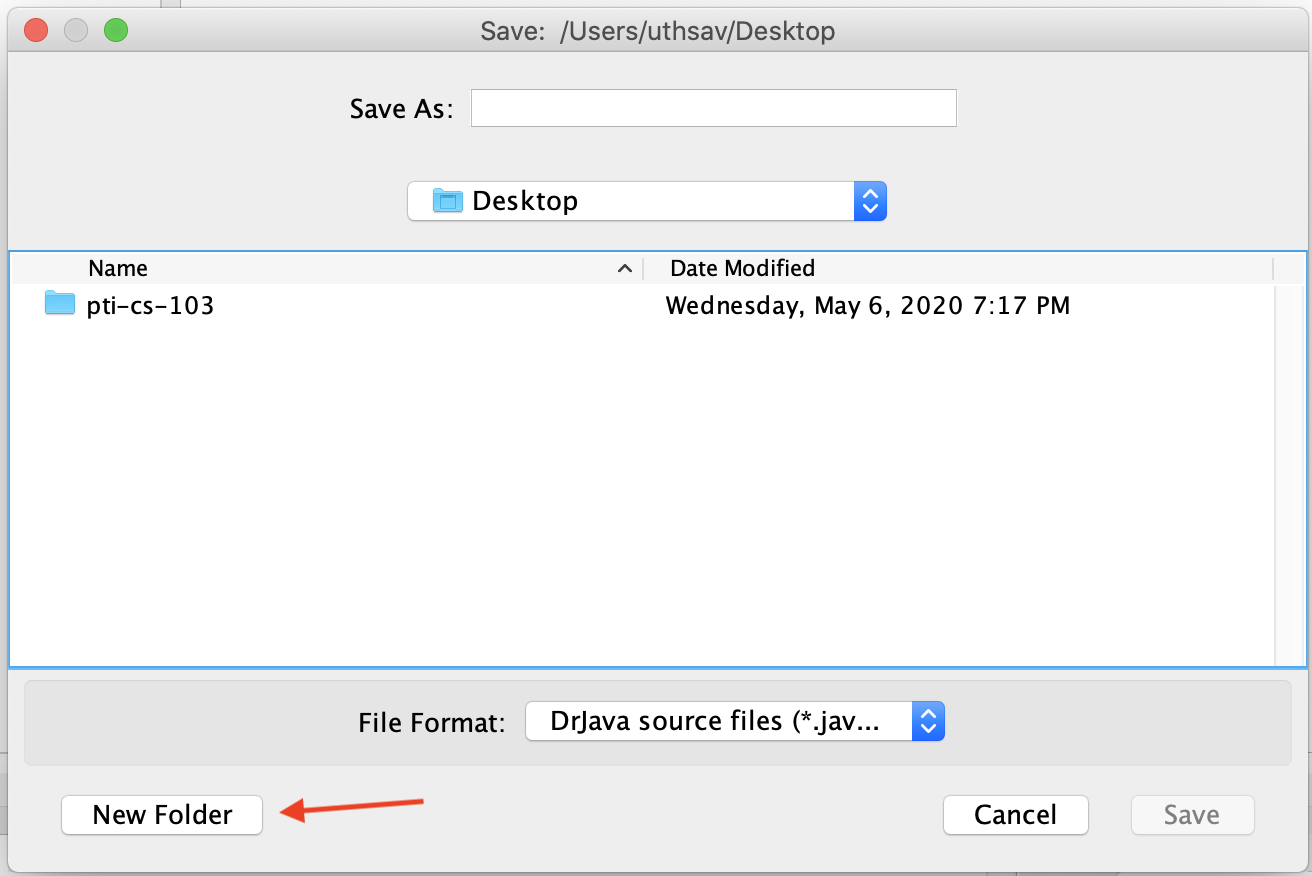
\includegraphics[width=0.85\textwidth]{images/hello_world_saving}
	\caption{Creating a CS103 folder inside your Desktop.}
	\label{fig:helloworld:sec:saving}
\end{figure}

Next, make another folder, called ``Chapter\_2", inside the CS103 folder for this class's assignment (see Figure \ref{fig:helloworld:sec:saving2}).

\begin{figure}[ht]
	\centering
	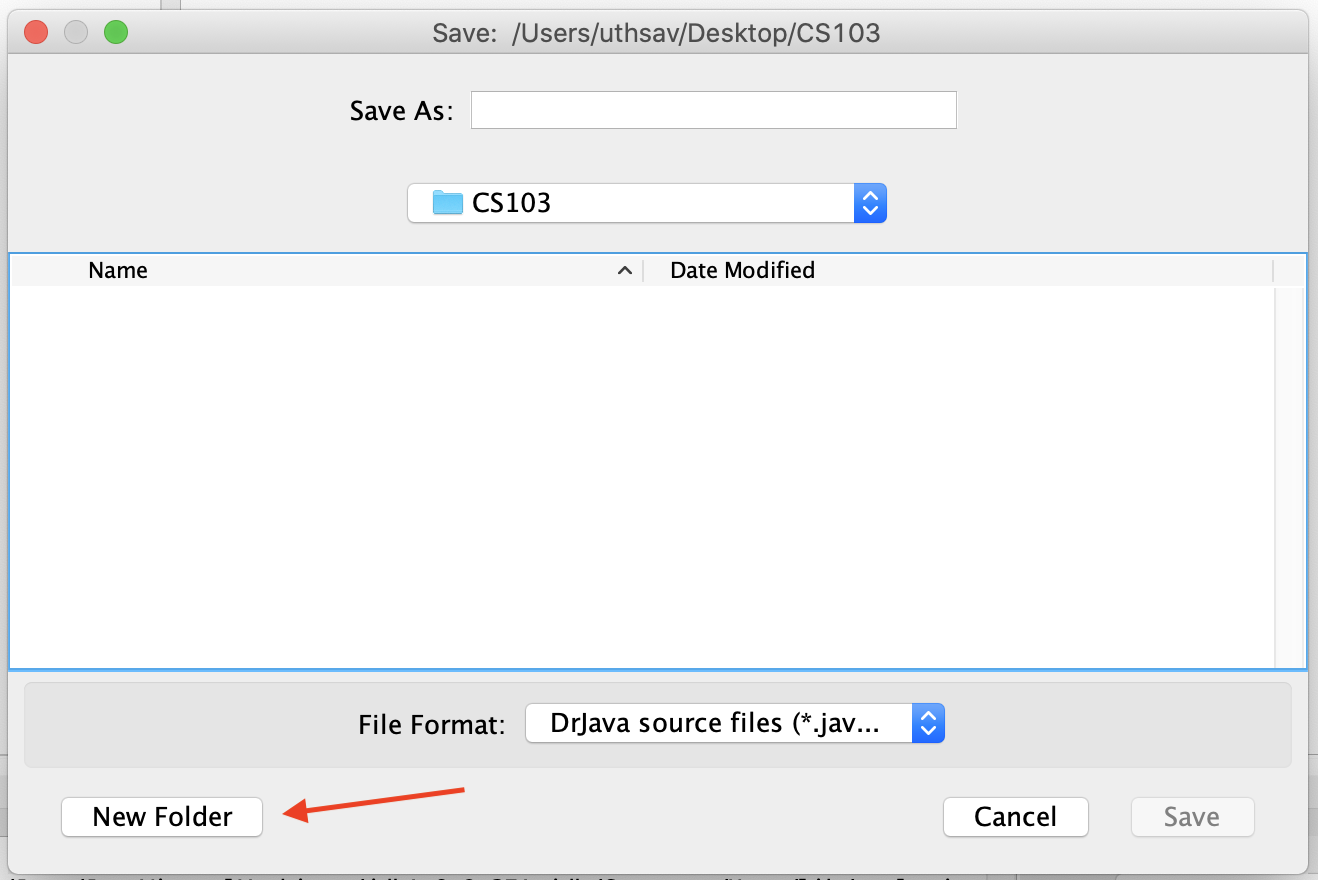
\includegraphics[width=0.85\textwidth]{images/hello_world_saving2}
	\caption{Creating another folder inside the CS103 folder.}
	\label{fig:helloworld:sec:saving2}
\end{figure}

Finally, save your file inside this folder with the filename \ic{HelloWorld.java}. The \ic{.java} file extension is used for code written in Java. 
Note that the file name for \ic{.java} files need to match the name of the class (for us, the name of our class is \ic{HelloWorld}).

Clicking the ``Compile'' button at the top will first save your file (if it hasn't already been saved) and then \emph{compile} it. Compiling converts your human-readable
source code into instructions that are easier for the computer to read. In Java, these instructions are in the form of a \ic{.class} file. After you click compile, DrJava will create a
\ic{HelloWorld.class} file which contains the instructions for the computer.


After clicking ``Compile,'' the bottom part of the window should say
\ic{Compilation completed.}

\subsection{Errors with compiling}

If there is a problem with your program, you might get an error message when you try compiling. Don't panic! Errors happen all the time --- even to experienced programmers. Fixing errors is known as \emph{debugging}, and is an incredibly valuable skill. Here we will look at two common errors, and how to fix them. 

For example, suppose we forgot to include the final curly brace, i.e. our code looked like the following.

\begin{code}
class HelloWorld {
    
    public static void main(String[] args) {
        System.out.println("Hello World!");
    }
\end{code}

If we hit the  ``Compile" button, then the bottom window should now show an error, with the message \ic{Error: reached end of file while parsing} (see below).

\begin{figure}[ht]
	\centering
	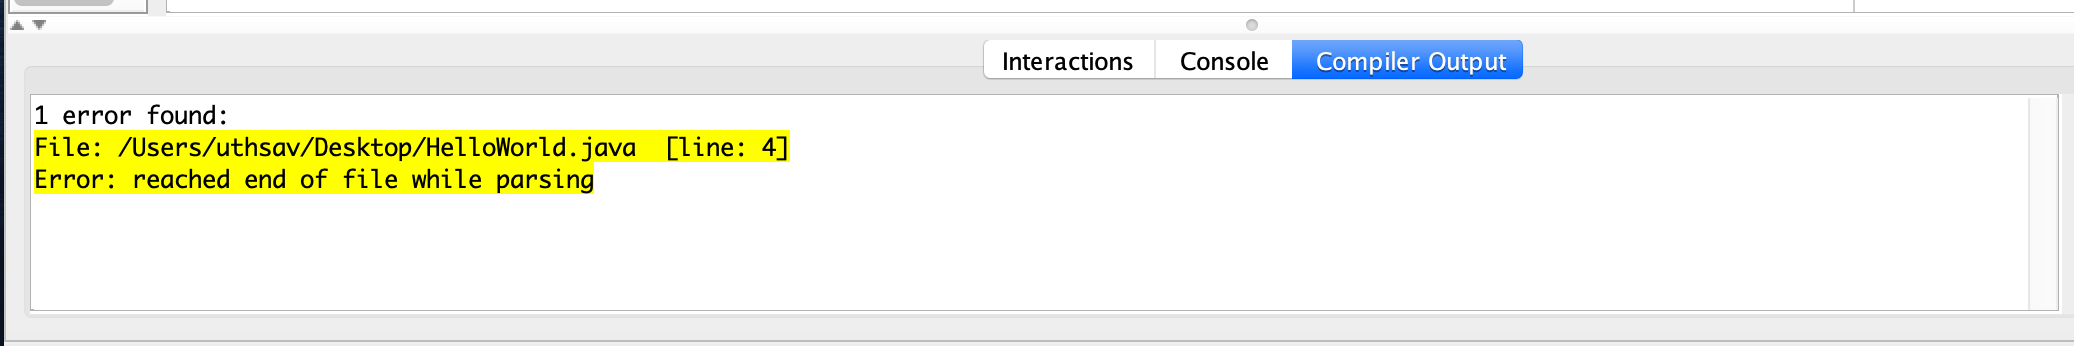
\includegraphics[width=0.85\textwidth]{images/hello_world_error.png}
	\caption{Example of compilation error when missing a curly bracket.}
	\label{fig:helloworld:sec:error}
\end{figure}

In general, \ic{Error: reached end of file while parsing} shows up if you did not pair every left curly brace \{ with a right curly brace \}.
To fix this error, add the last curly brace \} back in and hit ``Compile'' again.
%Note that in the bottom part of the window, the ``Compiler Output'' tab is selected. This tab is where you can view any messages from compilation.

Another common error is forgetting to end a command with a \;. For example, suppose your code looks like the following.

\begin{code}
class HelloWorld {
    
    public static void main(String[] args) {
        System.out.println("Hello World!")
    }
}
\end{code}

Note that Line 4 does not end with a semicolon. If we hit the ``Compile" button, the bottom window will show the error message \ic{Error: ';' expected}.

\begin{figure}[ht]
	\centering
	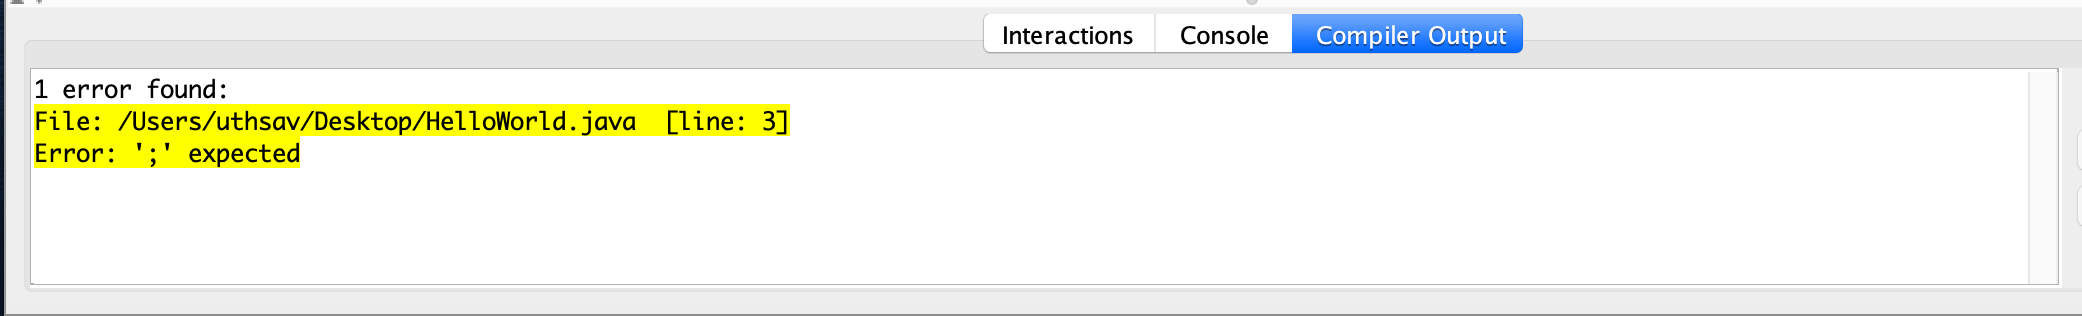
\includegraphics[width=0.85\textwidth]{images/hello_world_error2.png}
	\caption{Example of compilation error when missing a semicolon.}
	\label{fig:helloworld:sec:error2}
\end{figure}

% Let's see another example of a compilation error. Try deleting the semicolon \ic{;} from the program and hit ``Compile.''
The message \ic{Error: ';' expected} arises because the curly brace on line 5 was reached without the semicolon being
encountered. In Java, every statement must end in a semicolon. In this case, the print statement on line 4 must
end in a semicolon. Add the semicolon back in and recompile the program. Compilation should succeed.

As you progress through the course, you will run into many errors in your programs. This is a normal part of being a programmer. Recognizing different kinds of errors, and knowing how to fix them, are important skills that you will develop in this course.

\section{Running Code with DrJava}
Now that the program has been written and compiled, it is time to run it.
We will use DrJava to run our compiled program by clicking the ``Run'' button in the toolbar. After clicking the ``Run" button, in the bottom part of the window, you should see the following. (If there are any errors, ask your teacher for assistance.)
\begin{code}
> run HelloWorld
Hello World!
>
\end{code}

If you made it this far, then congrats! You ran your first program.

In the bottom window, the \ic{run HelloWorld} part indicates that you want to run the program \ic{HelloWorld}. The following line is the output of the program. 

Note that in the bottom part of the window, the ``Interactions'' tab is now
selected. This tab allows you to interact with your program. Clicking
the ``Run'' button is equivalent to clicking the ``Interactions'' tab, typing
\ic{run HelloWorld}, and then hitting enter/return key on your keyboard.

If you would like, you can type \ic{run HelloWorld} after the final \ic{>} and
type the enter/return key to run your program again.

\section{Making Changes}
Now we've successfully written, compiled, and ran our first Java program.
As an exercise, let's make our ``Hello World!'' more enthusiastic.
\newline

\textbf{Exercise.} Change the \ic{Hello World!} in line 4 to \ic{Hello World!!}. Compile and re-run your program.
\newline

 In general,
you can make changes to your program, recompile it, and run it again
to see the results of your changes.

\subsection{Adding comments to your code}

It is sometimes helpful to provide explanations of what your code is doing. These are known as \emph{comments}. We will look at a few ways to comment your ``Hello World!" program.

Try adding \ic{ //print hello} to the end of line 4, so that your line 4 now looks like this:
\begin{code}
        System.out.println("Hello World!!"); // print hello
\end{code}

Now compile and run your program. The behavior should remain unchanged from the previous time you ran the program.

The two forward slashes \ic{//} denote the beginning of an \emph{inline comment}. Comments are ignored by the compiler and do not have any effect on
the program's behavior. They are
useful for adding explanations or providing information to people that are reading the code. In this case,
the comment \ic{print hello} is explaining the purpose of the code on that line.

Now try adding \ic{//} to the beginning of line 4, so that it looks as follows:
\begin{code}
//        System.out.println("Hello World!!"); //print hello
\end{code}
Now compile and run your program. You should find that there is now no output. The two forward slashes that you added turned the whole line into a comment. As far as the compiler is concerned, your program is the same
as if the entire line 4 did not exist.This is sometimes called ``commenting out" your code. In DrJava, a shortcut for commenting out a line is to hit ''control" and "/" simultaneously.

\subsection{Multiple print statements}

Uncomment line 4 by deleting the forward slashes you added at the beginning of it.
Now add the following lines after line 4:
\begin{code}
System.out.println("Hello!"); // print hello again
System.out.println("Goodbye World!"); // say goodbye
\end{code}
Your code now has \emph{multiple statements}. In particular, you now have three. The first one on line 4 will print
\ic{Hello World!!}, the second one will print \ic{Hello!}, and the third will print \ic{Goodbye World!}.
Note that each of these statements is followed by a semicolon.
Deleting any one of these semicolons will result in a compilation error (give it a try!).
Your code should now look as follows:
\begin{code}
class HelloWorld {
    
    public static void main(String[] args) {
        System.out.println("Hello World!!"); //print hello
        System.out.println("Hello!"); // print hello again
        System.out.println("Goodbye World!"); // say goodbye
    }
    
}
\end{code}
Try compiling it and running it. The output should look as follows:
\begin{code}
Hello World!!
Hello!
Goodbye World!
\end{code}

\subsection{Block comments}

Let's add some description of what we're doing by adding a \emph{block comment}.
A block comment begins with \ic{/*} and is ended whenever \ic{*/} is encountered.
It may (but does not necessarily need to) span multiple lines.
Right before the main method, add a block comment to get the following:
\begin{code}
class HelloWorld {

    /* Main method to print out the following:
         Hello World!!
         Hello!
         Goodbye World!
    */
    public static void main(String[] args) {
        System.out.println("Hello World!!"); //print hello
        System.out.println("Hello!"); // print hello again
        System.out.println("Goodbye World!"); // say goodbye
    }

}
\end{code}
If you compile and run the program now, it should have the same behavior as before, since whatever occurs
inside comments does not affect the program's behavior.

Inline comments can be nested inside block comments, so for example, the following program
will compile without issue:
\begin{code}
class HelloWorld {

    /* Main method to print out the following:
         Hello World!!
         Hello!
         Goodbye World!
    */
    public static void main(String[] args) {
        /*
        System.out.println("Hello World!!"); //print hello
        System.out.println("Hello!"); // print hello again
        System.out.println("Goodbye World!"); // say goodbye
        */
    }

}
\end{code}
Note that since we have commented out all the code in the main method,
this program is actually the same as the following program that we considered earlier:
\begin{code}
class HelloWorld {

    public static void main(String[] args) {
//        System.out.println("Hello World!!"); //print hello
    }

}
\end{code}

\subsection{Understanding whitespace}

Let's now consider the following program that has two print statements and no comments:
\begin{code}
class HelloWorld {

    public static void main(String[] args) {
        System.out.println("Hello!");
        System.out.println("Goodbye!");
    }

}
\end{code}
Try compiling and running the program. Note the output.
What happens when we remove the linebreaks and spaces between each pair of print statements?
Try removing them to get the following:
\begin{code}
class HelloWorld {

    public static void main(String[] args) {
        System.out.println("Hello!");System.out.println("Goodbye!");
    }

}
\end{code}
Now compile and run the program. What happens?
The behavior should still be such that it prints the same output:
\begin{code}
Hello!
Goodbye!
\end{code}
\emph{Whitespace} such as linebreaks and spaces do not have any meaning in Java.
While spaces are necessary to separate things like \ic{class} and \ic{HelloWorld} or \ic{String[]} and \ic{args}
so that Java can distinguish between them, spaces are otherwise unimportant.
Linebreaks have no significance at all in a Java program except to denote when an inline comment
should end.

That being said, whitespace should be used to make your code more legible. Although you can write
all your Java programs on a single line, it is considered very bad style!
For demonstrative purposes, here the original Hello World Java program all on two lines:
\begin{code}
class HelloWorld{public static void main(String[] args)
    {System.out.println("Hello World!");}}
\end{code}
Try compiling and running it. It should print \ic{Hello World!} as its output.
You can get rid of all the spacing after the close parenthesis \ic{)} to get it all on one line--it
just doesn't fit on the page if it's all on one line here!
